%LTeX: language=pt-br
% !TeX root = Apostila_IM381.tex

\cleardoublepage
\section{Revisão modelo de barra}

    Nesta seção, será apresentada uma revisão do modelo de barra, sua equação diferencial, com alguns exemplos e exercícios.

    \subsection{Hipóteses}

        As principais hipóteses do modelo de barra são:

        \begin{itemize}
            \item Estrutura esbelta - comprimento muito maior que sua largura ou espessura;
            \item Material linear elástico isotrópico;
            \item Pequenas deformações e pequenos deslocamentos;
            \item Submetido apenas a cargas ao longo do seu comprimento;
            \item Deformações locais desprezíveis (princípio de Saint-Venant).
        \end{itemize}

        A última hipótese está relacionada ao princípio de Saint-Venant. Este afirma que, dado um conjunto de forças aplicada em uma parte da superfície de um corpo, tal que sua força e momento resultantes são nulos, então os efeitos de deformação devido a esta deve ser ínfima em regiões suficientemente distantes (Figura \ref{fig:venant}). Para a barra, isto implica em um perfil de forças uniforme.

        \begin{figure}[h!]
            \centering
            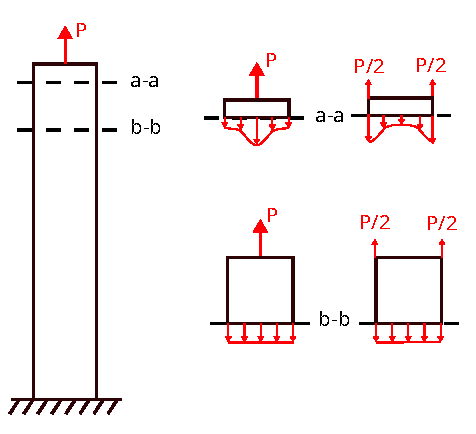
\includegraphics[scale=1]{Figures/2-Resmat/Venant.pdf}
            \caption{Princípio de Saint-Venant. Forças com mesma resultante possuem os mesmos efeitos se estivermos suficientemente distantes de seu ponto de aplicação.}
            \label{fig:venant}
        \end{figure}

    \subsection{Dedução da equação diferencial}

        Considere uma barra com uma área da seção transversal variável $A(x)$, sujeita a uma força distribuída $p(x)$. Fazendo de um elemento infinitesimal desta estrutura (Figura \ref{fig:barra}), podemos calcular o seu equilíbrio de forças:

        \begin{figure}[h!]
            \centering
            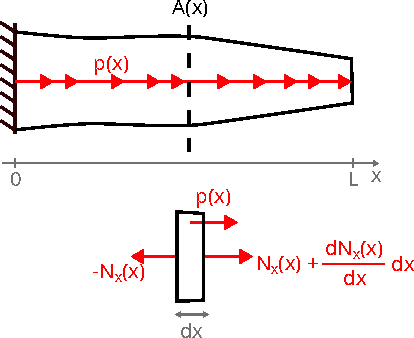
\includegraphics[scale=1]{Figures/2-Resmat/Bar.pdf}
            \caption{Equilíbrio de uma barra. Elemento infinitesimal da barra em equilíbrio.}
            \label{fig:barra}
        \end{figure}

        \begin{equation*}
            \sum F_x = 0
        \end{equation*}

        \begin{equation*}
            \frac{dN_x}{dx} = -p(x)
        \end{equation*}


        Conforme mencionado anteriormente, podemos considerar que os esforços internos ao longo da seção tranversal são uniformes. Portanto, a tensão normal $\sigma_{xx}$ é constante ao longo da largura e espessura:

        \begin{equation*}
            \int_A \sigma_{xx}(x) dA = N_x(x)
        \end{equation*}

        \begin{equation}
            \sigma_{xx}(x) = \frac{N_x(x)}{A(x)}
        \end{equation}


        Como o material é considerado linear elástico e isotrópico, podemos correlacionar as tensões com as deformações pela Lei de Hooke, a partir do Módulo de Young $E(x)$ do material:

        \begin{equation}
            \sigma_{xx}(x) = E(x)\varepsilon_{xx}(x)
        \end{equation}

        Finalmente, como os deslocamentos e as deformações são pequenas, os deslocamentos axiais $u(x)$ podem ser escritos como:

        \begin{equation}
            \frac{du(x)}{dx} = \varepsilon_{xx}(x)
        \end{equation}

        Juntando todas as expressões anteriores, chega-se à equação diferencial da barra:

        \begin{equation}
            \frac{d}{dx}\left(E A \frac{du}{dx}\right) = -p(x)
        \end{equation}

        Se considerarmos uma barra com seção transversal e módulo de elasticidade uniformes, chegamos à expressão simplificada:

        \begin{equation}
            E A \frac{d^2u}{dx^2} = -p(x)
        \end{equation}


        Esta equação deve ser resolvida com o auxílio de condições de contorno. Estas podem ser de dois principais tipos: condição de Dirichlet ou de Neumann. As condições de contorno de Dirichlet são condições no deslocamento na extremidade do domínio. Por exemplo, para uma barra de comprimento $L$ da Figura \ref{fig:barra_exemplo1}, com $x \in \left(0,L\right)$, podemos impor que $u(0) = u_0$. As condições de Neumann são condições na força aplicadas na extremidade do domínio. Por exemplo, para a mesma barra que a anterior, podemos aplicar uma força $F$ de tração na extremidade direita da barra. Neste caso, $N_x(L) = F$. Os sinais desta condição de contorno devem seguir o diagrama da Figura \ref{fig:convencao_normal}. Note que, embora usualmente estes diagramas sejam chamados de ``convenção da Resmat'', estes não são definidos arbitrariamente, mas são provenientes dos cálculos do equilíbrio.

        \begin{figure}[h!]
            \centering
            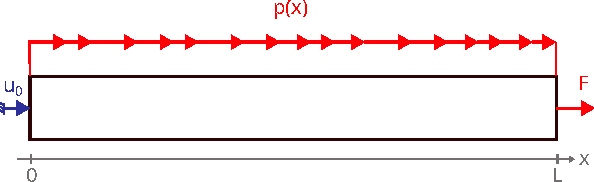
\includegraphics[scale=1]{Figures/2-Resmat/Barra_exemplo.pdf}
            \caption{Exemplo de barra com deslocamento imposto à esquerda e força aplicada à direita.}
            \label{fig:barra_exemplo1}
        \end{figure}

        \begin{figure}[h!]
            \centering
            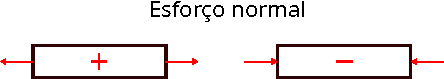
\includegraphics[scale=1]{Figures/2-Resmat/Esforcos.pdf}
            \caption{Convenção de sinais para esforços normais}
            \label{fig:convencao_normal}
        \end{figure}

        Desta forma, chega-se à seguinte equação diferencial para a barra (para este exemplo de condições de contorno):

        \begin{equation}
            \left\{
            \begin{array}{l}
                E A \frac{d^2u}{dx^2} = -p(x)\\
                u(0) = u_0\\
                N_x(L) = \left.EA\frac{du}{dx}\right|_{x=L} = F
            \end{array}
            \right.
        \end{equation}


    \subsection{Solução por funções de singularidade}
    \label{sec:singularidade}

        Para resolver a equação diferencial analiticamente, é necessário representar as forças como uma função $p(x)$. Entretanto, em muitos casos, a força não será contínua, como no caso de forças concentradas. Para representar essas forças, são usadas \textbf{funções de singularidade}.

        As funções de singularidade, de forma geral, são representadas por $\left\langle x-a \right\rangle^n$, modificando $a$ e $n$. Para representar uma força concentrada, podemos usar a função delta de Dirac. A função delta de Dirac é a função impulso unitário $\delta_a(x)$, conforme mostrado na Figura \ref{fig:dirac}, com o intervalo $\Delta$ sendo levado ao seu limite zero, tal que:

        \begin{figure}[h!]
            \centering
            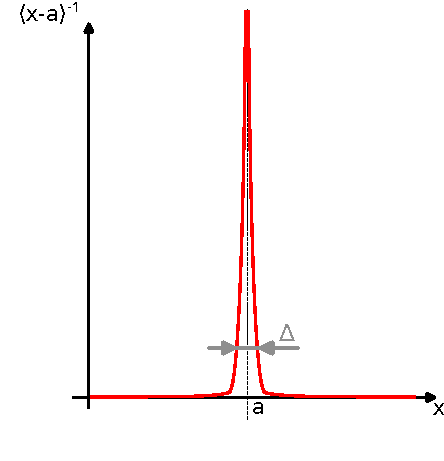
\includegraphics[scale=1]{Figures/2-Resmat/Dirac.pdf}
            \caption{Função impulso unitário.}
            \label{fig:dirac}
        \end{figure}

        \begin{equation*}
            \delta_a(x) = \left\{\begin{array}{l}
                0, x \neq a\\
                \text{não definido}, x=a
            \end{array}
            \right.
        \end{equation*}

        \begin{equation*}
            \int_{-\infty}^{\infty} \delta_a(x) dx = 1
        \end{equation*}

        No contexto de funções de singularidade, esta é $\delta_a(x) = \left\langle x-a\right\rangle^{-1}$

        Sua integral é a função degrau unitário (ou função Heaviside):

        \begin{equation*}
            H(x) = \left\langle x-a\right\rangle^0
            =
            \begin{array}{l}
                0, x < a\\
                1, x > a
            \end{array}
        \end{equation*}

        A partir de $n=0$, temos funções nulas para $x<a$ e polinomiais para $x\geq a$:

        \begin{equation*}
            \left\langle x-a\right\rangle^n =
            \left\{
            \begin{array}{l}
                0, x < a\\
                \left(x-a\right)^n, x > a
            \end{array}
            \right.
            \quad , n \in \left\{1,2, \ldots \right\}
        \end{equation*}

        A Figura \ref{fig:singularidade} ilustra algumas funções de singularidade.

        \begin{figure}[h!]
            \centering
            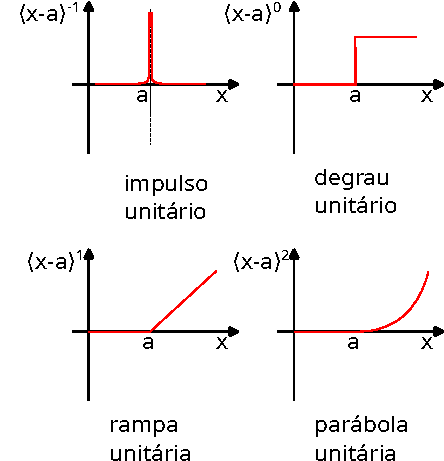
\includegraphics[scale=1.4]{Figures/2-Resmat/Singularidade.pdf}
            \caption{Funções de singularidade}
            \label{fig:singularidade}
        \end{figure}

        As derivadas das funções de singularidade podem, portanto, ser escrita da seguinte forma:

        \begin{equation*}
            \frac{d}{dx}\left\langle x-a\right\rangle^n =
            \left\{
            \begin{array}{l}
                \left\langle x-a\right\rangle^{n-1}, n \leq 0\\
                n\left\langle x-a\right\rangle^{n-1}, n > 0
            \end{array}
            \right.
        \end{equation*}

        As funções de singularidade podem ser usadas, portanto, para representar não apenas forças unitárias, mas também para forças distribuídas quaisquer no domínio. Na próxima seção, serão mostrados alguns exemplos de solução de problemas de barra por funções de singularidade.

    \subsection{Exemplos}

        \subsubsection{Exemplo 1:}

        Encontre o campo de deslocamento, os esforços internos e as reações de apoio da barra da Figura \ref{fig:barra_ex1}. Suponha $EA = 10^{3} N$.

        \begin{figure}[h!]
            \centering
            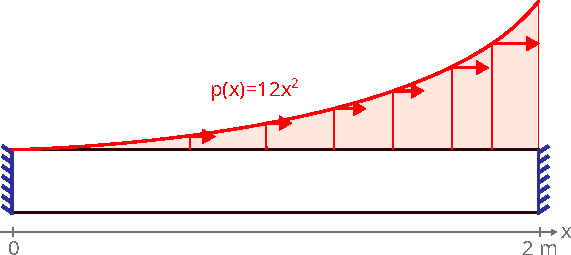
\includegraphics[scale=1]{Figures/2-Resmat/Exemplo1.pdf}
            \caption{Barra do Exemplo 1}
            \label{fig:barra_ex1}
        \end{figure}


        \subsubsection*{Solução:}

        O sistema está engastado nas duas extremidades, logo $u(0) = u(2) = 0$. A força distribuída pode ser escrita como:

        \begin{equation*}
            p(x) = 12x^2
        \end{equation*}

        Portanto, a equação diferencial é:

        \begin{equation*}
            \left\{
            \begin{array}{l}
                EAu''(x) = -12x^2\\
                u(0) = 0\\
                u(2) = 0
            \end{array}
            \right.
        \end{equation*}

        Para resolver, integramos sucessivamente a equação:

        \begin{equation*}
            EAu''(x) = -12x^2
        \end{equation*}

        \begin{equation*}
            EAu'(x) = -4x^3 + C_1
        \end{equation*}

        \begin{equation*}
            EAu(x) = -x^4 + C_1 x + C_2
        \end{equation*}

        \begin{equation*}
            u(x) = \frac{1}{EA} \left[-x^4 + C_1 x + C_2\right]
        \end{equation*}

        \noindent no qual as constantes $C_1$ e $C_2$ surgem da integração. Para obtê-las, aplicamos as condições de contorno:


        \begin{equation*}
            u(0) = 0 \rightarrow EAu(0) = -0^4 + C_1 0 + C_2 = 0
        \end{equation*}
        
        \begin{equation*}
            C_2 = 0
        \end{equation*}

        \begin{equation*}
            u(2) = 0 \rightarrow EAu(2) = -2^4 + 2C_1 = 0
        \end{equation*}

        \begin{equation*}
            C_1 =-8 N
        \end{equation*}

        Portanto:

        \begin{equation*}
            u(x) = \frac{1}{10^{3}} \left[-x^4 + 8 x\right] [m]
        \end{equation*}

        \begin{equation*}
            u(x) = -x^4 + 8 x [mm]
        \end{equation*}

        O esforço interno é:
        
        \begin{equation*}
            N_x(x) = EAu'(x) = -4x^3 + 8 [N]
        \end{equation*}

        As Figuras \ref{fig:ex1_barra_ux} e \ref{fig:ex1_barra_Nx} mostram as curvas do deslocamento e esforço normal. As reações de apoio são encontradas pelo esforço interno nas extremidades, usando também a convenção da Figura \ref{fig:convencao_normal}:

        \begin{figure}[h!]
            \centering
            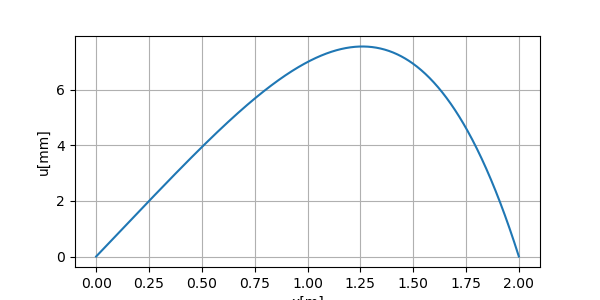
\includegraphics[scale=1]{Figures/2-Resmat/deslocamento_ex1.png}
            \caption{Campo de deslocamento do Exemplo 1}
            \label{fig:ex1_barra_ux}
        \end{figure}

        \begin{figure}[h!]
            \centering
            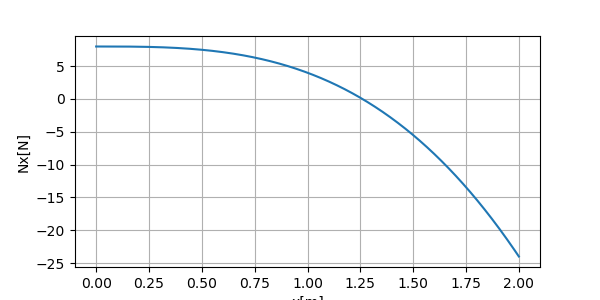
\includegraphics[scale=1]{Figures/2-Resmat/esforco_ex1.png}
            \caption{Esforço normal do Exemplo 1}
            \label{fig:ex1_barra_Nx}
        \end{figure}

        \begin{equation*}
            N_x(0) = 8 N
        \end{equation*}

        \begin{equation*}
            N_x(2) = -24 N
        \end{equation*}

        Na extremidade esquerda, pela convenção, o sinal positivo da condição de contorno é para a esquerda, portanto a força $N_x(0)$ deve apontar para a esquerda. Da mesma forma, na extremidade direita, o positivo é para a direita, portanto $N_x(2)$ deve apontar no sentido oposto, para a esquerda:

        \begin{equation*}
            R_A = -8N
        \end{equation*}

        \begin{equation*}
            R_B = -24N
        \end{equation*}

        Finalmente, se quiséssemos a deformação e a tensão, usaríamos:

        \begin{equation*}
            \sigma_{xx}(x) = \frac{N_x(x)}{A} = \frac{1}{A} \left[-4x^3 + 8\right]
        \end{equation*}

        \begin{equation*}
            \varepsilon_{xx}(x) = \frac{\sigma_{xx}}{E} = \frac{1}{EA} \left[-4x^3 + 8\right]
        \end{equation*}



        \subsubsection{Exemplo 2:}

        Encontre o campo de deslocamento, os esforços internos e as reações de apoio da barra da Figura \ref{fig:barra_ex2}. Suponha $EA = 10^{3} N$.

        \begin{figure}[h!]
            \centering
            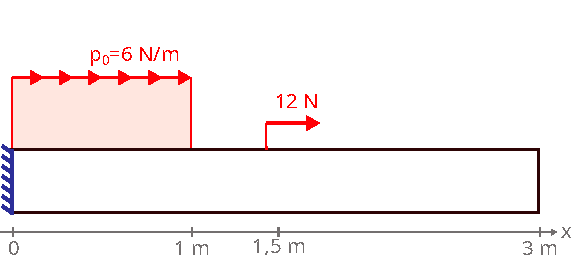
\includegraphics[scale=1]{Figures/2-Resmat/Exemplo2.pdf}
            \caption{Barra do Exemplo 2}
            \label{fig:barra_ex2}
        \end{figure}


        \subsubsection*{Solução}

        As condições de contorno neste problema são o engaste à esquerda ($u(0) = 0$) e a ausência de forças à direita ($N_x(3) = EAu'(3) = 0$).

        Para escrever $p(x)$, usaremos as funções de singularidade. A força distribuída pode ser escrita como a soma de uma força distribuída constante ao longo de todo o domínio com uma que anula com ela a partir de $x=1$ (Figura \ref{fig:barra_ex2_soma_forc}). A força concentrada é representada pelo delta de Dirac, multiplicado pela sua amplitude $12$ N:

        \begin{figure}[h!]
            \centering
            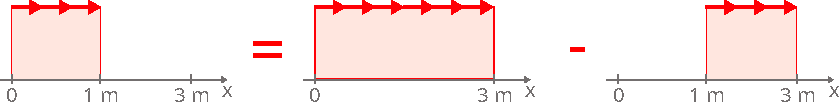
\includegraphics[scale=1]{Figures/2-Resmat/Soma_forc.pdf}
            \caption{Montagem da força distribuída}
            \label{fig:barra_ex2_soma_forc}
        \end{figure}

        \begin{equation*}
            p(x) = 6 - 6\sing{x}{1}{0} + 12\sing{x}{1,5}{-1}
        \end{equation*}


        Portanto, temos a equação diferencial:

        \begin{equation*}
            \left\{
            \begin{array}{l}
                EAu''(x) = -6 + 6\sing{x}{1}{0} - 12\sing{x}{1,5}{-1}\\
                u(0) = 0\\
                EAu'(3) = 0
            \end{array}
            \right.
        \end{equation*}


        Integrando sucessivamente:

        \begin{equation*}
            EAu''(x) = -6 + 6\sing{x}{1}{0} - 12\sing{x}{1,5}{-1}
        \end{equation*}

        \begin{equation*}
            EAu'(x) = -6x + 6\sing{x}{1}{1} - 12\sing{x}{1,5}{0} + C_1
        \end{equation*}

        \begin{equation*}
            EAu(x) = -3x^2 + 3\sing{x}{1}{2} - 12\sing{x}{1,5}{1} + C_1 x + C_2
        \end{equation*}

        \begin{equation*}
            u(x) = \frac{1}{EA} \left[-3x^2 + 3\sing{x}{1}{2} - 12\sing{x}{1,5}{1} + C_1 x + C_2\right]
        \end{equation*}

        Aplicando as condições de contorno:

        \begin{equation*}
            u(0) = 0 \rightarrow EAu(0) = C_2 = 0
        \end{equation*}

        \begin{equation*}
            EAu'(3) = 0 \rightarrow EAu'(3) = -6 \cdot 3 + 6\sing{3}{1}{1} - 12\sing{3}{1,5}{0} + C_1 = 0
        \end{equation*}

        \begin{equation*}
           -18 + 12 - 12 + C_1 = 0 \rightarrow C_1 = 18 N
        \end{equation*}


        Portanto:

        \begin{equation*}
            u(x) = \frac{1}{10^3} \left[-3x^2 + 3\sing{x}{1}{2} - 12\sing{x}{1,5}{1} + 18 x\right] [m]
        \end{equation*}

        \begin{equation*}
            u(x) = -3x^2 + 3\sing{x}{1}{2} - 12\sing{x}{1,5}{1} + 18 x [mm]
        \end{equation*}

        Perceba que $u(x)$ é uma função definida por trechos (já substituindo e fazendo as distributivas):

        \begin{equation*}
            u(x) = 
            \left\{
            \begin{array}{cl}
                -3x^2 + 18x &, x<1\\
                12x + 3 &, 1\leq x<1,5\\
                21 &, x\geq 1,5\\
            \end{array}
            \right. [mm]
        \end{equation*}


        O esforço normal:

        \begin{equation*}
            N_x(x) = EAu'(x) = -6x + 6\sing{x}{1}{1} - 12\sing{x}{1,5}{0} + 18
        \end{equation*}

        \begin{equation*}
            N_x(x) = 
            \left\{
            \begin{array}{cl}
                -6x + 18 &, x<1\\
                12 &, 1\leq x<1,5\\
                0 &, x\geq 1,5\\
            \end{array}
            \right. [N]
        \end{equation*}

        As Figuras \ref{fig:ex2_barra_ux} e \ref{fig:ex2_barra_Nx} mostram as curvas do deslocamento e esforço interno. A reação de apoio é dado por:

        \begin{figure}[h!]
            \centering
            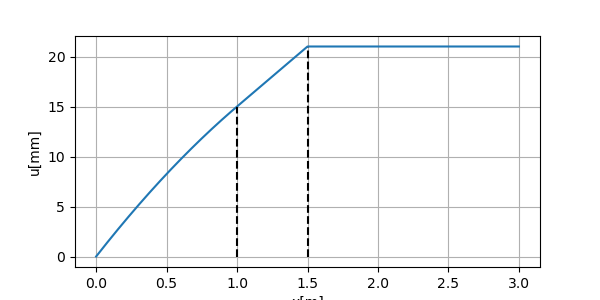
\includegraphics[scale=1]{Figures/2-Resmat/deslocamento_ex2.png}
            \caption{Campo de deslocamento do Exemplo 2}
            \label{fig:ex2_barra_ux}
        \end{figure}

        \begin{figure}[h!]
            \centering
            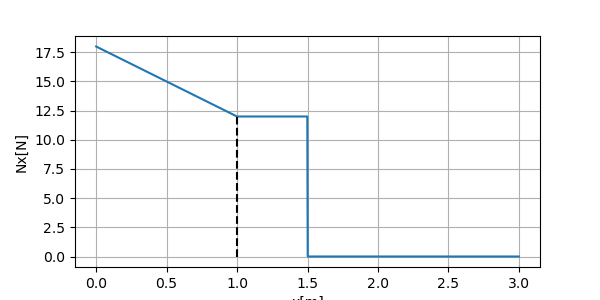
\includegraphics[scale=1]{Figures/2-Resmat/esforco_ex2.png}
            \caption{Esforço normal do Exemplo 2}
            \label{fig:ex2_barra_Nx}
        \end{figure}

        \begin{equation*}
            N_x(0) = -6 \cdot 0 + 18 = 18 N
        \end{equation*}

        Como a reação é positiva para a esquerda, na extremidade esquerda, então:

        \begin{equation*}
            R_A = -18 N
        \end{equation*}
    
        


